\chapter{NAO Kinematics: The Solution}
\label{approach}

As mentioned in Chapter~\ref{related}, the existing approaches to kinematics for the NAO robot are not completely suitable for our needs. We seek to find a solution to the forward kinematics problem for any set of joint values as input and not only for the current joint values. In addition, we seek to find a real-time analytical solution for the problem of inverse kinematics without any approximations. In the sections below, we describe our solutions to both of these problems.


\section{Forward Kinematics for the NAO Robot}


Aldebaran Robotics provides the DH parameters for each kinematic chain of the robot in the documentation~\cite{AldebaranNaoDoc}. However, our experimentation with the provided values revealed that the given parameters for the arm chains are incorrect. Therefore, we found our own parameters for the arms and we used the provided parameters for the legs and the head.


\subsubsection*{NAO Zero Position}
We must define the base frame of the robot and the zero position of the joints before we proceed. The base frame is taken to be the torso frame; Figure~\ref{fig:torso} shows the axes of this frame. The same figure shows also the zero position of all the joints of the robot, which is the one provided by Aldebaran Robotics. As we can see, in this position the ShoulderRoll joints are not really roll joints, but are yaw joints, so we can understand that the names of the joints do not necessarily describe the actual movement of the joint in the base frame given the zero position.

\begin{figure}[h]
\begin{center}
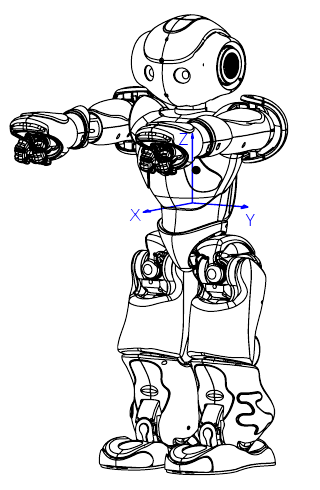
\includegraphics[height = 10cm]{Figures/torso_frame.png}
\caption{Base (torso) frame and zero position of the joints}
\label{fig:torso}
\end{center}
\end{figure}


\subsubsection*{Notation}
We provide a brief description of the symbols we use in our math calculations. All matrices used are affine transformation matrices of three types: $T$ is a transformation matrix, $R_x, R_y, R_z$ are basic rotations matrices, and $A$ is a translation matrix. The subscript of a symbol refers to the start frame and the superscript refers to the destination frame. The torso is the point where all the kinematic chains begin and is located at the center of the NAO body. ``Base'' is the start frame of the chain (the torso frame), while ``End'' is the end effector of the chain. The numbers appearing as subscripts or superscripts refer to the joints in the current kinematic chain, numbered consistently with the ordering given in the tables of Chapter~\ref{problem}. Also, we denote the initialization of a translation matrix as $A(d_x,d_y,d_z)$ and of rotation matrices as $R_x(\theta_x)$, $R_y(\theta_y)$, or $R_z(\theta_z)$.

We present the DH parameters of each kinematic chain in a separate table and, besides the DH parameters, we provide the translations from the ``Base'' to the first joint and from the last joint to the ``End''. Finally, we provide some necessary rotations to adjust the frame of the last joint to the frame of the end effector (``End'').


\subsubsection*{Forward Kinematics Equations}
Forward kinematics for each chain of the NAO robot is a transformation that maps a point from the frame of the last joint to the base frame. In our case, the end effector is the point of interest. Forward kinematics are defined in terms of transformation, rotation, and translation matrices, and the final result is a single transformation matrix that maps points from one frame to another. 

\subsubsection*{Extracting the Point in the Three-Dimensional Space}
The result of forward kinematics is an affine transformation matrix $T$ with the $X$ block being a rotation matrix and the $Y$ block being a translation vector. We need to extract the $(p_x, p_y, p_z)$ position and the $(a_x,a_y,a_z)$ orientations of the final point. The position $(p_x, p_y, p_z)$ can be simply read off the translation part of the transformation matrix:
\begin{align*}
p_x &= T_{(1,4)}\\
p_y &= T_{(2,4)}\\
p_z &= T_{(3,4)}
\end{align*}
The rotation of the final transformation table is a $R_zR_yR_x$ rotation table, whose analytical form is shown in Section~\ref{sec:affine}. Now it's easy to extract the orientation $(a_x,a_y,a_z)$:
\begin{align*}
a_x &= \arctan\!2 \left(T_{(3,2)},T_{(3,3)}\right)\\
a_y &= \arctan\!2 \left(-T_{(3,1)},\sqrt{{T_{(3,2)}}^2 + {T_{(3,3)}}^2}\right)\\
a_z &= \arctan\!2 \left(T_{(2,1)},T_{(1,1)}\right)
\end{align*}

\subsection{Forward Kinematics for the Head}
The head is the simplest kinematic chain of the NAO robot, but it has two useful end effectors, namely the top and the bottom cameras. Table~\ref{tab:DHhead} shows the DH parameters for the head chain. Now, we can combine these matrices to find the point of the end effector in the frame space of the torso:
\[
T^\text{End}_\text{Base} = A^0_\text{Base}T^1_0T^2_1R_x(\tfrac{\pi}{2})R_y(\tfrac{\pi}{2})A^\text{End}_{2}
\]
$T^1_0$ and $T^2_1$ are the DH transformation matrices of the corresponding joints (HeadYaw, HeadPitch). $A^\text{End}_{2}$ is one of the two translation matrices given in Table~\ref{tab:DHhead} for the two end effectors (top and bottom camera). The point of the end effector in the three-dimensional space of the torso can be extracted from $T^\text{End}_\text{Base}$.


\begin{table}[t!]
\centering
\caption{DH parameters for the head chain of the NAO robot}
\label{tab:DHhead}
\begin{tabular}{|l|>{\centering\arraybackslash}m{2.55cm}|>{\centering\arraybackslash}m{2.55cm}|>{\centering\arraybackslash}m{2.55cm}|>{\centering\arraybackslash}m{2.55cm}|}
\hline
\textbf{Frame (Joint)} & $\mathbf{a}$ & $\boldsymbol{\alpha}$ & $\mathbf{d}$ & $\boldsymbol{\theta}$\\ \hline
Base & \multicolumn{4}{c|}{$A(0,0,\text{\footnotesize{NeckOffsetZ}})$} \\ \hline
HeadYaw & $0$ & $0$ & $0$ & $\theta_1$ \\ \hline
HeadPitch & $0$ & $-\frac{\pi}{2}$ & $0$ & $\theta_2 - \frac{\pi}{2}$ \\ \hline
Rotation & \multicolumn{4}{c|}{$R_x(\frac{\pi}{2})R_y(\frac{\pi}{2})$} \\ \hline
Top Camera & \multicolumn{4}{c|}{$A(\text{\footnotesize{topCameraX}},0,\text{\footnotesize{topCameraZ}})$} \\ \hline
Bottom Camera & \multicolumn{4}{c|}{$A(\text{\footnotesize{bottomCameraX}},0,\text{\footnotesize{bottomCameraZ}})$} \\ \hline
\multicolumn{5}{|c|}{\footnotesize{topCameraX=53.9mm, topCameraZ=67.9mm, bottomCameraX=48.8mm, bottomCameraZ=23.8mm}} \\ \hline
\end{tabular}
\end{table}

\subsection{Forward Kinematics for the Left Arm}

The kinematic chain for the left arm consists of four joints. So, we need to find four sets of DH parameters, one for each joint. First, we must move from the torso to the base of the joint and we can do that with a simple translation along the $y$-axis and the $z$-axis. After that, we must align the coordinate frame with the rotation axis of the first joint (LShoulderPitch). So, we rotate about the $x$-axis of the coordinate frame by $-\frac{\pi}{2}$, thus the $\alpha$ parameter for LShoulderPitch is $-\frac{\pi}{2}$, while $d$, $a$ are $0$. Now, we must rotate the coordinate frame again to become aligned with the rotation axis of the second joint (LShoulderRoll). So, we rotate about the $x$-axis by $\frac{\pi}{2}$, thus the $\alpha$ parameter for LShoulderRoll is $\frac{\pi}{2}$, while $d$, $a$ are $0$. Next, we need to align the coordinate frame with the rotation axis of the third joint (LElbowYaw). To do so, we must rotate about the $y$-axis. The DH parameters do not directly encode a rotation about the $y$-axis, so we must first rotate about the $z$-axis and then about the $x$-axis to effectively realize a rotation about the $y$-axis. Thus, we add $\frac{\pi}{2}$ to the angle $\theta_2$ of the previous joint (to rotate about the $z$-axis) and then rotate about the $x$-axis by $\frac{\pi}{2}$ (the $\alpha$ parameter of LElbowYaw). Also, we must move ElbowOffsetY towards the $x_2$ axis so the parameter $a$ is ElbowOffsetY. Then, we move along the $z$-axis to reach the position of the LElbowYaw joint, so its $d$ parameter is set to UpperArmLength. Finally, for the fourth joint (LElbowRoll) we rotate about the $x$-axis by $-\frac{\pi}{2}$, thus the $\alpha$ parameter for LElbowRoll is $-\frac{\pi}{2}$, while $d$, $a$ are $0$. At the end, we only need a simple rotation to fix the orientation of our coordinate frame and a simple translation to reach the end effector.



\begin{table}[t!]
\centering
\caption{DH parameters for the left arm chain of the NAO robot}
\label{tab:DHlarm}
\begin{tabular}{|l|>{\centering\arraybackslash}m{2.55cm}|>{\centering\arraybackslash}m{2.55cm}|>{\centering\arraybackslash}m{2.55cm}|>{\centering\arraybackslash}m{2.55cm}|}
\hline
\textbf{Frame (Joint)} & $\mathbf{a}$ & $\boldsymbol{\alpha}$ & $\mathbf{d}$ & $\boldsymbol{\theta}$\\ \hline
Base & \multicolumn{4}{c|}{$A(0,\text{\footnotesize{ShoulderOffsetY}},\text{\footnotesize{ShoulderOffsetZ}})$} \\ \hline
LShoulderPitch & $0$ & $-\frac{\pi}{2}$ & $0$ & $\theta_1$ \\ \hline
LShoulderRoll & $0$ & $\frac{\pi}{2}$ & $0$ & $\theta_2 + \frac{\pi}{2}$ \\ \hline
LElbowYaw & \footnotesize{ElbowOffsetY} & $\frac{\pi}{2}$ & \footnotesize{UpperArmLength} & $\theta_3$ \\ \hline
LElbowRoll & $0$ & $-\frac{\pi}{2}$ & $0$ & $\theta_4$ \\ \hline
Rotation & \multicolumn{4}{c|}{$R_z(-\frac{\pi}{2})$} \\ \hline
End effector & \multicolumn{4}{c|}{$A(\text{\footnotesize{HandOffsetX+LowerArmLength}},0,0)$} \\ \hline
\end{tabular}
\end{table}

Table~\ref{tab:DHlarm} shows the DH parameters for all the joints of the left arm chain along with the necessary translations and rotations.
Now, we can easily calculate the final transformation matrix:
\[
T^\text{End}_\text{Base} = A^0_\text{Base}T^1_0T^2_1T^3_2T^4_3R_z(-\tfrac{\pi}{2})A^\text{End}_{4}
\]

\subsection{Forward Kinematics for the Right Arm}
The kinematic chain of the right arm is fully symmetric with the left arm chain relatively to the plane defined by the $x$-axis and the $z$-axis. So, the differences between the two chains are only in the distances along the $y$-axis and in the joints that rotate about the $y$-axis. Also, in this chain we must add one extra rotation matrix after the final translation, because the $z$-axis is inverted. All the DH parameters for this chain can be seen in Table~\ref{tab:DHrarm} and the final transformation matrix is:
\[
T^\text{End}_\text{Base} = A^0_\text{Base}T^1_0T^2_1T^3_2T^4_3R_z(-\tfrac{\pi}{2})A^\text{End}_{4}
\]

\begin{table}[!t]
\centering
\caption{DH parameters for the right arm chain of the NAO robot}
\label{tab:DHrarm}
\begin{tabular}{|l|>{\centering\arraybackslash}m{2.55cm}|>{\centering\arraybackslash}m{2.55cm}|>{\centering\arraybackslash}m{2.85cm}|>{\centering\arraybackslash}m{2.55cm}|}
\hline
\textbf{Frame (Joint)} & $\mathbf{a}$ & $\boldsymbol{\alpha}$ & $\mathbf{d}$ & $\boldsymbol{\theta}$\\ \hline
Base & \multicolumn{4}{c|}{$A(0,\text{\footnotesize{$-$ShoulderOffsetY}},\text{\footnotesize{ShoulderOffsetZ}})$} \\ \hline
RShoulderPitch & $0$ & $-\frac{\pi}{2}$ & $0$ & $\theta_1$ \\ \hline
RShoulderRoll & $0$ & $\frac{\pi}{2}$ & $0$ & $\theta_2 + \frac{\pi}{2}$ \\ \hline
RElbowYaw & $-$\footnotesize{ElbowOffsetY} & $\frac{\pi}{2}$ & \footnotesize{UpperArmLength} & $\theta_3$ \\ \hline
RElbowRoll & $0$ & $-\frac{\pi}{2}$ & $0$ & $\theta_4$ \\ \hline
Rotation & \multicolumn{4}{c|}{$R_z(-\frac{\pi}{2})$} \\ \hline
End effector & \multicolumn{4}{c|}{$A(\text{\footnotesize{HandOffsetX+ LowerArmLength}},0,0)$} \\ \hline
\end{tabular}
\end{table}



\subsection{Forward Kinematics for the Left Leg}
The kinematic chain for the left leg has six joints and it is the longest chain on the NAO robot. The DH parameters for these joints are interesting, because of the ``weird'' orientation of the HipYawPitch joint. Table~\ref{tab:DHlleg} shows the DH parameters for the entire kinematic chain of the left leg and the final transformation matrix is:
\[
T^\text{End}_\text{Base} = A^0_\text{Base}T^1_0T^2_1T^3_2T^4_3T^5_4T^6_5R_z(\pi)R_y(-\tfrac{\pi}{2})A^\text{End}_{6}
\]

\begin{table}[!t]
\centering
\caption{DH parameters for the left leg chain of the NAO robot}
\label{tab:DHlleg}
\begin{tabular}{|l|>{\centering\arraybackslash}m{2.55cm}|>{\centering\arraybackslash}m{2.55cm}|>{\centering\arraybackslash}m{2.55cm}|>{\centering\arraybackslash}m{2.55cm}|}
\hline
\textbf{Frame (Joint)} & $\mathbf{a}$ & $\boldsymbol{\alpha}$ & $\mathbf{d}$ & $\boldsymbol{\theta}$\\ \hline
Base & \multicolumn{4}{c|}{$A(0,\text{\footnotesize{HipOffsetY}},\text{\footnotesize{$-$HipOffsetZ}})$} \\ \hline
LHipYawPitch & $0$ & $-\frac{3\pi}{4}$ & $0$ & $\theta_1 - \frac{\pi}{2}$ \\ \hline
LHipRoll & $0$ & $-\frac{\pi}{2}$ & $0$ & $\theta_2 + \frac{\pi}{4}$ \\ \hline
LHipPitch & $0$ & $\frac{\pi}{2}$ & $0$ & $\theta_3$ \\ \hline
LKneePitch & \footnotesize{$-$ThighLength} & $0$ & $0$ & $\theta_4$ \\ \hline
LAnklePitch & \footnotesize{$-$TibiaLength} & $0$ & $0$ & $\theta_5$ \\ \hline
LAnkleRoll & $0$ & $-\frac{\pi}{2}$ & $0$ & $\theta_6$ \\ \hline
Rotation & \multicolumn{4}{c|}{$R_z(\pi)R_y(-\tfrac{\pi}{2})$} \\ \hline
End effector & \multicolumn{4}{c|}{$A(0,0,\text{\footnotesize{$-$FootHeight}})$} \\ \hline
\end{tabular}
\end{table}



\subsection{Forward Kinematics for the Right Leg}
Similarly to the arms, the kinematic chains for the legs are fully symmetric relatively to the plane defined by the $x$-axis and the $z$-axis. So, the differences between the two chains is only in the distances along the $y$-axis and in the joints that rotate about the $y$-axis. Table~\ref{tab:DHrleg} shows all the DH parameters for the right leg chain and the final transformation matrix is: 
\[
T^\text{End}_\text{Base} = A^0_\text{Base}T^1_0T^2_1T^3_2T^4_3T^5_4T^6_5R_z(\pi)R_y(-\tfrac{\pi}{2})A^\text{End}_{6}
\]

\begin{table}[!t]
\centering
\caption{DH parameters for the right leg chain of the NAO robot}
\label{tab:DHrleg}
\begin{tabular}{|l|>{\centering\arraybackslash}m{2.55cm}|>{\centering\arraybackslash}m{2.55cm}|>{\centering\arraybackslash}m{2.55cm}|>{\centering\arraybackslash}m{2.55cm}|}
\hline
\textbf{Frame (Joint)} & $\mathbf{a}$ & $\boldsymbol{\alpha}$ & $\mathbf{d}$ & $\boldsymbol{\theta}$\\ \hline
Base & \multicolumn{4}{c|}{$A(0,\text{\footnotesize{$-$HipOffsetY}},\text{\footnotesize{$-$HipOffsetZ}})$} \\ \hline
RHipYawPitch & $0$ & $-\frac{\pi}{4}$ & $0$ & $\theta_1 - \frac{\pi}{2}$ \\ \hline
RHipRoll & $0$ & $-\frac{\pi}{2}$ & $0$ & $\theta_2 - \frac{\pi}{4}$ \\ \hline
RHipPitch & $0$ & $\frac{\pi}{2}$ & $0$ & $\theta_3$ \\ \hline
RKneePitch & \footnotesize{$-$ThighLength} & $0$ & $0$ & $\theta_4$ \\ \hline
RAnklePitch & \footnotesize{$-$TibiaLength} & $0$ & $0$ & $\theta_5$ \\ \hline
RAnkleRoll & $0$ & $-\frac{\pi}{2}$ & $0$ & $\theta_6$ \\ \hline
Rotation & \multicolumn{4}{c|}{$R_z(\pi)R_y(-\tfrac{\pi}{2})$} \\ \hline
End effector & \multicolumn{4}{c|}{$A(0,0,\text{\footnotesize{$-$FootHeight}})$} \\ \hline
\end{tabular}
\end{table}


\subsection{Forward Kinematics for Combined Chains}
The forward kinematics transformations presented above assume the torso frame as the base frame. In practice, a NAO user may be interested in finding the point of the torso relatively to one of the feet. Note that this is the forward kinematics problem for the reverse chain. Given that the forward kinematics transformation matrices are affine transformation matrices, we can obtain the solution for this reverse problem by simply inverting the corresponding transformation matrix. 
For example, inverting the transformation matrix for the left leg chain yields a transformation matrix for the point of the torso in the frame of the left foot: 
\[
T^\text{Torso}_\text{LFoot} = {\left(T^\text{LFoot}_\text{Torso}\right)}^{-1}
\]
This solution reversion property of the forward kinematics allows the combination of multiple chains to obtain the point of the end effector of one chain in the frame of the end effector of the other chain through their common point (torso). 

For example, it is possible to find the point of the head relatively to the left foot. The kinematic chains for the head and for the left leg are relative to the torso frame. So, by inverting the transformation matrix of the left leg chain, we locate the torso relatively to the left foot frame. Then, we just multiply with the transformation matrix of the head chain and obtain a new transformation matrix that describes the point of the head relatively to the left foot frame.
\[
T^\text{Head}_\text{LFoot} = {\left(T^\text{LFoot}_\text{Torso}\right)}^{-1}T^\text{Head}_\text{Torso}
\]
This property is extremely useful, because we can describe any end effector relatively to the frame of any other end effector. For example, with this, we can find the exact height of the camera from the ground.

\subsection{Calculation of the Center Of Mass}
The Center of Mass (CoM) of a body in the three-dimensional space is a position, which corresponds to the weighted average location of all the mass in the body. From a physics point of view, the body (even if oddly-shaped) could be represented by a point mass located at the CoM. In humanoid robots, knowledge of the CoM is important to maintain balance. It is easy to see that the CoM changes, as the joint values change and the kinematic chains move in the three-dimensional space. 

The NAO robot consists of a group of connected parts (joints and the corresponding links). Each part has its own known mass and its own (local) CoM at a known static position. For any given configuration of the robot, forward kinematics can be applied to locate each of these parts in the three-dimensional space of the torso frame and from there calculate the exact position of the robot CoM relatively to the torso frame. 

Aldebaran Robotics provides the information needed for CoM calculations, in particular the mass of the whole robot and the masses of all parts of the robot. The mass of each distinct part is referenced by the corresponding joint of that part and its own local CoM is given relatively to its own joint frame.

The CoM of the entire robot is calculated relatively to the torso frame and the calculation order is simple. We first construct smaller kinematic chains, one for each of the 21 joints. Each of these smaller kinematic chains terminates at the corresponding joint and the position of the local CoM is set to be the end effector. We compute the forward kinematics for each of these 21 chains. Then, we extract the translation block of each transformation matrix and we multiply it with the mass of the corresponding part/joint. In total, we have 21 chains plus the torso chain (a zero-length chain). Finally, we add all the individual weighted translation matrices and the result is divided by the total mass of the robot. The outcome of this calculation is the position of the CoM relatively to the torso frame.











\section{Inverse Kinematics for the NAO Robot}


Forward kinematics can find the point of an end effector, relatively to the start frame, given the values of the joints. Now, we turn our attention to the inverse problem: find a set of values for the joints that drive a given end effector to a desired point relatively to the torso frame. The inverse kinematics presented below solve the problem for the five kinematic chains that start at the robot torso.

A point of the end effector in the three-dimensional space consists of a position $(p_x,p_y,p_z)$ and an orientation $(a_x,a_y,a_z)$. As mentioned above, the outcome of forward kinematics is an affine transformation matrix, which includes a rotation block and a translation block. The rotation block $R$ takes the form $R_zR_yR_x$. Thus, we can construct the complete transformation matrix $T$ from the base frame to the point of the end effector mentioned above:
\[
\begin{small}
T = 
\begin{bmatrix}
\cos a_y\cos a_z & -\cos a_x\sin a_z + \sin a_x\sin a_y\cos a_z & \sin a_x\sin a_z + \cos a_x\sin a_y\cos a_z & p_x\\
\cos a_y\sin a_z & \cos a_x\cos a_z + \sin a_x\sin a_y\sin a_z & -\sin a_x\cos a_z + \cos a_x\sin a_y\sin a_z & p_y\\
-\sin a_y & \sin a_x\cos a_y & \cos a_x\cos a_y & p_z\\
0 & 0 & 0 & 1
\end{bmatrix}
\end{small}
\]
Given $T$, our goal now is to find a set of joint values that leads to the same transformation through the kinematic chain. As mentioned before, the problem of inverse kinematics cannot be solved without the solution of forward kinematics. This is true, because the equations we must solve to find the values of the joints are formed by writing down the forward kinematics transformation matrix symbolically with the $\theta_i$'s of the DH parameters appearing as symbols in the matrix. This symbolic matrix is set to be equal to $T$ to yield twelve non-linear equations with the values $\theta_i$ of the $n$ joints of the chain as unknowns. In fact, we will have a total of $2n$ unknowns, because all the $\theta_i$'s appear inside a sine or a cosine, therefore for each joint $i$ there are two dependent unknowns in the system, $\sin\theta_i$ and $\cos\theta_i$.

As we shall see below, we obtain some of the solutions using $\arccos$ and $\arcsin$. The problem is that $\arcsin$ returns an angle in $\left[-\tfrac{\pi}{2},+\tfrac{\pi}{2}\right]$ and $\arccos$ returns an angle in $\left[0,\pi\right]$, even though the possible values of a joint can be in the range $\left[-\pi,+\pi\right]$. Thus, if $\theta^*_i$ is a value returned by $\arcsin$ or $\arccos$ as a solution, there is one additional symmetric solution, $\pi - \theta^*_i$ for $\arcsin$ and $-\theta^*_i$ for $\arccos$. Due to these symmetries, the equations lead to a small number of distinct candidate solutions, some of which may be infeasible or invalid because of the constrained range of each joint. To determine a valid and correct solution, we simply run each one of these solutions through the forward kinematics to verify that indeed the end effector of the chain reaches the desired position and orientation. Invalid solutions are discarded and only correct ones are kept. 

In summary, the solution methodology we followed to solve the inverse kinematics problem includes the following steps: 
\begin{enumerate}
%\itemsep 6pt
\item Construct the (numeric) transformation matrix to the target point
\item Construct the (symbolic) transformation matrix through the chain
\item Form a non-linear system by equating the two matrices 
\item Manipulate both sides to make the problem easier
\item Find values for some joints through geometry and trigonometry
\item Find values for the remaining joints from the non-linear system
\item Validate all candidate solutions through forward kinematics
\end{enumerate}
This methodology is quite generic and can be used in solving the problem for any kinematic chain of up to six DOF. Some steps of this methodology appear in the literature, however to our knowledge no previous work has employed all these seven steps together. 


\subsection{Inverse Kinematics for the Head}
The head chain consists of only two joints, therefore we can work either with the position $(p_x,p_y,p_z)$ or with the orientation $(a_x,a_y,a_z)$ of the target point to obtain a solution. In the latter case, we can achieve the desired target orientation simply by setting the HeadYaw and HeadPitch joints to $a_z$ and $a_y$ respectively. In the former case, we first construct the symbolic matrix from forward kinematics along the head chain:
\[
T = 
\begin{bmatrix}
-\cos\theta_1\sin\widehat{\theta}_2 & -\sin\theta_1 & \cos\theta_1\cos\widehat{\theta}_2 &  l_2\cos\theta_1\cos\widehat{\theta}_2 - l_1\cos\theta_1\sin\widehat{\theta}_2\\
-\sin\theta_1\sin\widehat{\theta}_2 & \cos\theta_1 & \cos\widehat{\theta}_2\sin\theta_1 & l_2\cos\widehat{\theta}_2\sin\theta_1 - l_1\sin\theta_1\sin\widehat{\theta}_2\\
-\cos\widehat{\theta}_2 & 0 & -\sin\widehat{\theta}_2 & l_3 - l_2\sin\widehat{\theta}_2 - l_1\cos\widehat{\theta}_2\\
0 & 0 & 0 & 1
\end{bmatrix}
\]
where $\widehat{\theta}_2$ is the DH parameter $\theta$ for the second joint, $l_1 =$ cameraX, $l_2 =$ cameraZ, and $l_3 =$ NeckOffsetZ.
Since we only know the position $(p_x,p_y,p_z)$, we cannot reconstruct the rotation block of the matrix, so we focus on the translation block. From the symbolic matrix, we have: 
\[
T_{(3,4)} = l_3 - l_2\sin\widehat{\theta}_2 - l_1\cos\widehat{\theta}_2 = p_z
\]
We know from trigonometry that: 
\[
a\sin\theta + b\cos\theta = \sqrt{a^2+b^2}\sin\left(\theta + \psi\right)
\]
\[
\psi=\arctan\left(\frac{b}{a}\right) + \left\{ 
  \begin{array}{l l}
    0 & \quad \text{if }a\geq0\\
    \pi & \quad \text{if }a<0\\
  \end{array} \right.
\]
Given that $l_2>0$, we can now calculate $\widehat{\theta}_2$ as follows:
\[
\widehat{\theta}_2 = \arcsin\left(\cfrac{-p_z+l_3}{\sqrt{{l_1}^2+{l_2}^2}}\right) - \arctan\left(\frac{l_1}{l_2}\right)
\]
Now the final joint value $\theta_2$ is $\theta_2 = \widehat{\theta}_2 + \frac{\pi}{2}$.  From now on, we substitute $\theta_2 - \frac{\pi}{2}$ in $\widehat{\theta}_2$. Now, we can easily extract $\theta_1$ from $T_{(1,4)}$:
\[
\theta_1 = \arccos\left(\cfrac{p_x}{l_2\cos\left(\theta_2 - \frac{\pi}{2}\right) - l_1\sin\left(\theta_2 - \frac{\pi}{2}\right) } \right)
\]
So, the final inverse kinematics equations for the head chain are:
\begin{align*}
\theta_2 &= \arcsin\left(\cfrac{- p_z + l_3}{ \sqrt{{l_1}^2+{l_2}^2} }\right) - \arctan\left(\frac{l_1}{l_2}\right) + \frac{\pi}{2}\\
\theta_2 &= \pi - \arcsin\left(\cfrac{- p_z + l_3}{ \sqrt{{l_1}^2+{l_2}^2} }\right) - \arctan\left(\frac{l_1}{l_2}\right) + \frac{\pi}{2}\\
\theta_1 &= \pm\arccos\left(\cfrac{p_x}{l_2\cos\left(\theta_2 - \frac{\pi}{2}\right) - l_1\sin\left(\theta_2 - \frac{\pi}{2}\right) } \right)
\end{align*}
provided a target position $(p_x,p_y,p_z)$ or 
\begin{align*}
\theta_1 &= a_z\\
\theta_2 &= a_y
\end{align*}
provided a target orientation $(a_x,a_y,a_z)$.

\subsection{Inverse Kinematics for the Left Arm}
The left arm chain is far more complicated than the head chain. First, we construct the symbolic transformation matrix for the left arm chain, then we remove from the chain the Base and End transformation together with the End rotation.
\[
T = A^0_\text{Base}T^1_0T^2_1T^3_2T^4_3R_z(\tfrac{\pi}{2})A^\text{End}_{4}
\]
\[
T' = \left(A_\text{Base}^0\right)^{-1}T\left(R_z(\tfrac{\pi}{2})\right)^{-1}\left(A_4^\text{End}\right)^{-1}
\]
Then we invert $T'$:
\[
T'' = \left(T'\right)^{-1}
\]
\begin{align*}
T'' &= \begin{bmatrix}
r_{11} & r_{12} & r_{13} & r_{14}\\
r_{21} & r_{22} & r_{23} & r_{24}\\
r_{31} & r_{32} & r_{33} & r_{34}\\
0 & 0 & 0 & 1
\end{bmatrix}\\
r_{11} &= \cos\theta_4 \sin\theta_1 \sin\theta_3 + 
 \cos\theta_1 (\cos\widehat{\theta}_2 \cos\theta_3 \cos\theta_4 - \sin\widehat{\theta}_2 \sin\theta_4)\\
r_{12} &= \cos\theta_3 \cos\theta_4 \sin\widehat{\theta}_2 + \cos\widehat{\theta}_2 \sin\theta_4\\
r_{13} &= -\cos\widehat{\theta}_2 \cos\theta_3 \cos\theta_4 \sin\theta_1 + \cos\theta_1 \cos\theta_4 \sin\theta_3 + 
 \sin\theta_1 \sin\widehat{\theta}_2 \sin\theta_4\\
r_{14} &= -l_1 \cos\theta_3 \cos\theta_4 + l_2 \sin\theta_4\\
r_{21} &= -\sin\theta_1 \sin\theta_3 \sin\theta_4 - 
 \cos\theta_1 (\cos\theta_4 \sin\widehat{\theta}_2 + \cos\widehat{\theta}_2 \cos\theta_3 \sin\theta_4)\\
r_{22} &= \cos\widehat{\theta}_2 \cos\theta_4 - \cos\theta_3 \sin\widehat{\theta}_2 \sin\theta_4\\
r_{23} &= \cos\theta_4 \sin\theta_1 \sin\widehat{\theta}_2 + (\cos\widehat{\theta}_2 \cos\theta_3 \sin\theta_1 - \cos\theta_1 \sin\theta_3) \sin\theta_4\\
r_{24} &= l_2 \cos\theta_4 + l_1 \cos\theta_3 \sin\theta_4\\
r_{31} &= \cos\theta_3 \sin\theta_1 - \cos\theta_1 \cos\widehat{\theta}_2 \sin\theta_3\\
r_{32} &= -\sin\widehat{\theta}_2 \sin\theta_3\\
r_{33} &= \cos\theta_1 \cos\theta_3 + \cos\widehat{\theta}_2 \sin\theta_1 \sin\theta_3\\
r_{34} &= l_1 \sin\theta_3
\end{align*}
where $\widehat{\theta}_2$ is the DH parameter $\theta$ for the second (LShoulderRoll) joint, $l_1 =$ ElbowOffsetY, $l_2 =$ UpperArmLength.

We can extract $theta_3$ from the resulted transformation matrix:
\[
	\theta_3 = \left\{
	\begin{array}{l}
	arcsin\left(\frac{T''_{(3,4)}}{l_1}\right)\\
	\pi-arcsin\left(\frac{T''_{(3,4)}}{l_1}\right)
	\end{array} \right.
\]

The next angle we can find is $\theta_4$, so we focus on equations from the symbolic matrix, where we only have $\theta_4$ and/or $\theta_3$ (now $\theta_3$ is a known variable). Using $T''_{(1,4)}$, we have:

\begin{align*}
T''_{(1,4)} &= -l_1 \cos\theta_3 \cos\theta_4 + l_2 \sin\theta_4 &\Leftrightarrow\\
\sin\theta_4 &= \frac{T''_{(1,4)} + l_2\cos\theta_3\cos\theta_4}{l_3}
\end{align*}

Now, we focus on $T_{24}$:
\begin{align*}
T''_{24} &= l_2 \cos\theta_4 + l_1 \cos\theta_3 \sin\theta_4 &\Leftrightarrow\\
T''_{24} &= l_2 \cos\theta_4 + l_1 \cos\theta_3\frac{T''_{(1,4)} + l_2\cos\theta_3\cos\theta_4}{l_3} &\Leftrightarrow\\
\cos\theta_4 \left( l_2^2+l_1^2\cos^2\theta_3 \right) &= l_3 T''_{(2,4)} - l_2T''_{(1,4)}\cos\theta_3 &\Leftrightarrow\\
\theta_4 &= \pm arccos\left( \frac{l_3 T''_{(2,4)} - l_2T''_{(1,4)}\cos\theta_3}{l_2^2+l_1^2\cos^2\theta_3} \right)
\end{align*}

Next we manipulate again our chain. Now bot DH-transformations for $\theta_3$ and $\theta_4$ can be removed from the chain so:
\[
T''' = T'\left(T_2^3\right)^{-1}\left(T_3^4\right)^{-1}
\]
Now the final two joint values can be easily extract:
\[
\widehat{\theta_2} = arctan\left(\frac{T'''_{(1,2)}}{T'''_{(2,2)}}\right)
\]
\[
\theta_2 = \widehat{\theta_2}-\frac{\pi}{2}
\]
\[
\theta_1 = arctan\left(\frac{T'''_{(3,1)}}{T'''_{(3,3)}}\right)
\]
At this point, we have multiple solution sets for all the joints of the left arm, but some of them may be invalid. We find the correct set(s) through a forward kinematics validation step. In summary, the final inverse kinematics equations for the left arm chain are:
\begin{align*}
T' &= \left(A_\text{Base}^0\right)^{-1}T\left(R_z(\tfrac{\pi}{2})\right)^{-1}\left(A_4^\text{End}\right)^{-1}\\
T'' &= \left(T'\right)^{-1}\\
\theta_3 &= \left\{
	\begin{array}{l}
	arcsin\left(\frac{T''_{(3,4)}}{l_1}\right)\\
	\pi-arcsin\left(\frac{T''_{(3,4)}}{l_1}\right)
	\end{array} \right.\\
\theta_4 &= \pm arccos\left( \frac{l_3 T''_{(2,4)} - l_2T''_{(1,4)}\cos\theta_3}{l_2^2+l_1^2\cos^2\theta_3} \right)\\
T''' &= T'\left(T_2^3\right)^{-1}\left(T_3^4\right)^{-1}\\
\theta_2 &= arctan\left(\frac{T'''_{(2,1)}}{T'''_{(2,2)}}\right)-\frac{\pi}{2}\\
\theta_1 &= arctan\left(\frac{T'''_{(1,3)}}{T'''_{(3,3)}}\right)
\end{align*}



\subsection{Inverse Kinematics for the Right Arm}

The right and left arms are symmetric, thus the solution for the right arm differs only in the distances along the $y$-axis and at the ``roll'' joints (RShoulderRoll, RElbowRoll). The only basic difference with the distances along the $y$-axis are with the ElbowOffsetY that now becomes negative, thus $l_1 = -$ElbowOffsetY.

It is clear that the chain for the right arm is the same as the chain for the left arm. 
As we can see, the changes don't have any impact in the solution given for the left arm, that is, no denominator becomes zero after these changes. So, according to the previous section, the final inverse kinematics equations for the right arm chain are:
\begin{align*}
T' &= \left(A_\text{Base}^0\right)^{-1}T\left(R_z(\tfrac{\pi}{2})\right)^{-1}\left(A_4^\text{End}\right)^{-1}\\
T'' &= \left(T'\right)^{-1}\\
\theta_3 &= \left\{
	\begin{array}{l}
	arcsin\left(\frac{T''_{(3,4)}}{l_1}\right)\\
	\pi-arcsin\left(\frac{T''_{(3,4)}}{l_1}\right)
	\end{array} \right.\\
\theta_4 &= \pm arccos\left( \frac{l_3 T''_{(2,4)} - l_2T''_{(1,4)}\cos\theta_3}{l_2^2+l_1^2\cos^2\theta_3} \right)\\
T''' &= T'\left(T_2^3\right)^{-1}\left(T_3^4\right)^{-1}\\
\theta_2 &= arctan\left(\frac{T'''_{(2,1)}}{T'''_{(2,2)}}\right)-\frac{\pi}{2}\\
\theta_1 &= arctan\left(\frac{T'''_{(1,3)}}{T'''_{(3,3)}}\right)
\end{align*}





\subsection{Inverse Kinematics for the Left Leg}
\label{invleftleg}

The kinematic chain of the left leg has six joints, so it is much more difficult to find a solution. Since the first three joints of the chain (LHipYawPitch,  LHipRoll, LHipPitch) have intersecting axes, the problem is possibly solvable. The symbolic matrix for this chain is too complicated, therefore in order to simplify it, we remove the known translations from the kinematic chain:
\[
T = A^0_\text{Base}T^1_0T^2_1T^3_2T^4_3T^5_4T^6_5R_z(\pi)R_y(-\tfrac{\pi}{2})A^\text{End}_6
\]
\[
\widehat{T} = {\left(A^0_\text{Base}\right)}^{-1}T{\left(A^\text{End}_6\right)}^{-1}
\]
Now, we have a chain from the base frame of the first joint to the (rotated) frame of the last joint. The first joint, LHipYawPitch, is by construction rotated by $-\frac{3\pi}{4} $ about the $ x $-axis with respect to the torso frame. We rotate the origin of the chain by $\frac{\pi}{4}$ about the $x$-axis to make the first joint (LHipYawPitch) a yaw joint (aligned with the $z$-axis):
\[
\widetilde{T} = R_x(\tfrac{\pi}{4})\widehat{T}
\]
Now, the end effector is the LAnkleRoll joint and the base is the rotated LHipYawPitch joint. The first four joints (LHipYawPitch, LHipRoll, LHipPitch, LKneePitch) affect the position and orientation of the end effector and the other two joints (LAnklePitch, LAnkleRoll) affect only its orientation. It would be convenient, if only three joints were affecting the position of the end effector, since we operate in the three-dimensional space. Thus, we invert the transformation matrix to form the reverse chain. Now only the LAnkleRoll, LAnklePitch, and LKneePitch joints affect the position:
\[
T' = {\left(\widetilde{T}\right)}^{-1}
\]
The resulting symbolic matrix is still quite complex, but for now we only need the translation block, which is relatively simple:
\begin{align*}
&r_{14} = l_2\sin\theta_5 - l_1\sin\left(\theta_4 + \theta_5\right)\\
&r_{24} = \left(l_2\cos\theta_5 + l_1 \cos\left(\theta_4 + \theta_5\right)\right)\sin\theta_6\\
&r_{34} = \left(l_2\cos\theta_5 + l_1 \cos\left(\theta_4 + \theta_5\right)\right)\cos\theta_6
\end{align*}
where $l_1 =$ ThighLength and $l_2 =$ TibiaLength.
We can now find $\theta_4$ the same way we found $\theta_4$ for the arms. We focus on the triangle formed by the leg with  ThighLength, TibiaLength, and the distance from the base to the end effector in the reverse chain as sides:
\[
d = \sqrt{\left(s_x-p'_x\right)^2 + \left(s_y-p'_y\right)^2 + \left(s_z-p'_z\right)^2}
\]
% MGL: Is this really the distance? Why do I think that s'_i must be 0 or p' =p?
where $(s_x, s_y, s_z) = (0,0,0)$ is the new origin and $(p'_x, p'_y, p'_z) = (T'_{(1,4)}, T'_{(2,4)}, T'_{(3,4)})$ is the position of the new target point. Now, we can use the law of cosines to find the interior angle $\theta'_4$ between the thigh and tibia sides of the triangle:
\[
\theta'_4 =\arccos\left(\frac{{l_1}^2 + {l_2}^2 - d^2}{2 l_1 l_2}\right)\\
\]
Since $\theta'_4$ represents an interior angle, whereas the LKneePitch joint is stretched in the zero position, the resulting angle $\theta''_4$ in this range is computed by:
\[
\theta''_4 = \pi - \theta'_4
\]
Since the range of the LKneePitch joint includes both positive and negative angles, we finally extract $\theta_4$ as:
\[
\theta_4 = \pm\theta''_4
\]
Next, we extract the $\theta_6$ angle from the translation block using $r_{24}$ and $r_{34}$:
\begin{align*}
\frac{r_{24}}{r_{34}} &= \frac{p'_y}{p'_z} &\Leftrightarrow \\
\frac{\left(l_2\cos\theta_5 + l_1 \cos\left(\theta_4 + \theta_5\right)\right)\sin\theta_6}{\left(l_2\cos\theta_5 + l_1 \cos\left(\theta_4 + \theta_6\right)\right) \cos\theta_6} &= \frac{p'_y}{p'_z} &\Leftrightarrow \\
\theta_6 &= \arctan\left(\frac{p'_y}{p'_z}\right)&\text{if} \left(l_2\cos\theta_5 + l_1 \cos\left(\theta_4 + \theta_5\right)\right) \neq 0
\end{align*}
Since we don't know $\theta_5$, we cannot determine in advance when this solution is valid. Figure~\ref{fig:unlocus} shows the locus of the equation $l_2\cos\theta_5 + l_1 \cos\left(\theta_4 + \theta_5\right) = 0$ in the space of the KneePitch ($\theta_4$) and AnklePitch ($\theta_5$) joints; in these configurations, which represent only a fraction of extreme values in the joint space, no unique solution can be extracted for $\theta_6$. Essentially, in these configurations, the position of the end effector of the reverse chain (the hip joints) falls on the rotation axis of first joint (LAnkleRoll) in the reverse chain and therefore the LAnkleRoll joint ($\theta_6$) has no effect on its position; an infinity of solutions exists, given that for any choice of $\theta_6$, there will be a corresponding set of choices for the hip joints that achieves the target orientation. In practice, even if one of these configurations shows up during the solution, a division by zero never occurs, because the {\tt atan2} function in our implementation simply returns a result of 0. We adopt the solution $\theta_6=0$, and we relay the problem of the target orientation to the hip joints; invalid solutions, if any, will be rejected by the validation step.

\begin{figure}[!h]
	\begin{center}
		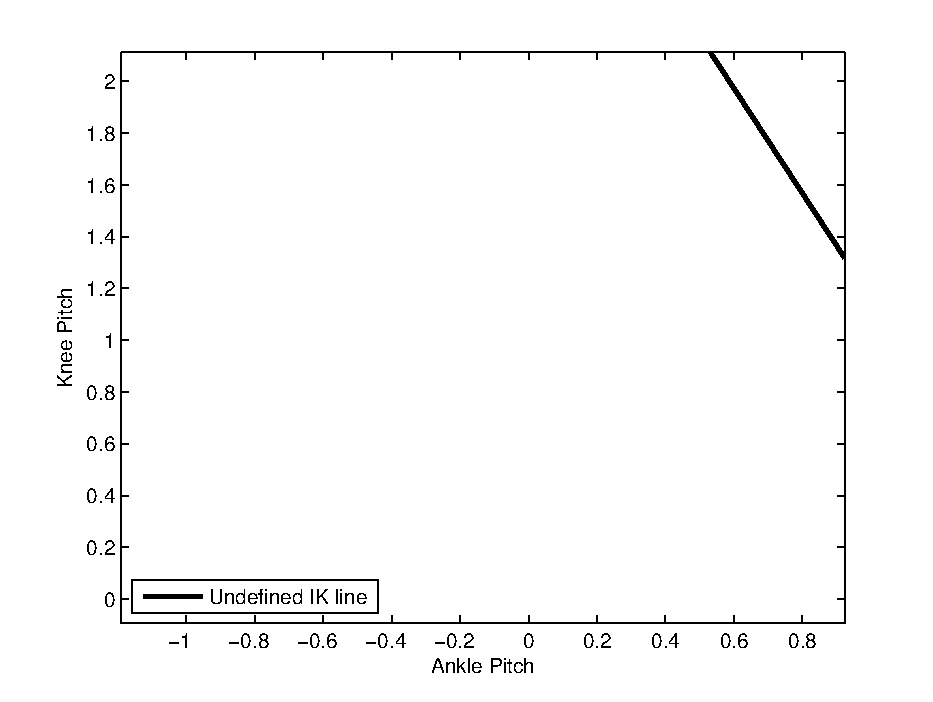
\includegraphics[height = 10cm]{Figures/locus.pdf}
 		\caption{Locus of leg configurations corresponding to non-unique solutions to $\theta_6$}
 		\label{fig:unlocus}
	\end{center}
\end{figure}

To move on, we go back to $\widetilde{T}$ and we remove the two rotations at the end of the chain along with the transformation $T^6_5$ which is now known, because $\theta_6$ is known:
\[
\widetilde{T}' = \widetilde{T}\left(T^6_5R_z\left(\pi\right)R_y(-\tfrac{\pi}{2})\right)^{-1}
\]
Like before, we form the reverse chain: 
\[
T'' = \left( \widetilde{T}' \right) ^{-1}
\]
and we extract the new target position $(p''_x, p''_y, p''_z) = (T''_{(1,4)}, T''_{(2,4)}, T''_{(3,4)})$. The translation block of the new symbolic transformation matrix is:
\begin{align*}
&r_{14} = l_2\cos\theta_5 + l_1\left(\cos\theta_5\cos\theta_4 - \sin\theta_5\sin\theta_4\right)\\
&r_{24} = -l_2\sin\theta_5 - l_1\left(\sin\theta_5\cos\theta_4 + \cos\theta_5\sin\theta_4\right)\\
&r_{34} = 0
\end{align*}
In these equations, $\theta_5$ is the only unknown. From $r_{14}$, we obtain an expression for $\cos\theta_5$:
\begin{align*}
r_{14} &= p''_x & \Leftrightarrow\\
\left(l_2+l_1\cos\theta_4\right) \cos\theta_5 &= p''_x + l_1\sin\theta_5\sin\theta_4 & \Leftrightarrow\\
\cos\theta_5 &= \cfrac{p''_x + l_1\sin\theta_5\sin\theta_4}{l_2+l_1\cos\theta_4}&\text{if }l_2+l_1\cos\theta_4\neq0
\end{align*}
Given the lengths of the links of the robot, the denominator $l_2+l_1\cos\theta_4$ becomes zero, only if $\cos\theta_4 = -1.029$, which is impossible, since $|\cos\theta_4| \le 1$. We continue with $r_{24}$: 
\begin{align*}
&\sin\theta_5\left(-l_2-l_1\cos\theta_4\right) - l_1\cos\theta_5\sin\theta_4 = p''_y& \Leftrightarrow\\
&\sin\theta_5\left(-l_2-l_1\cos\theta_4\right) - l_1\cfrac{p''_x + l_1\sin\theta_5\sin\theta_4}{l_2+l_1\cos\theta_4}\sin\theta_4\ =p''_y & \Leftrightarrow\\
&-\sin\theta_5\left(l_2+l_1\cos\theta_4\right) - \cfrac{l_1p''_x\sin\theta_4}{l_2+l_1\cos\theta_4} - \cfrac{{l_1}^2\sin\theta_5\sin^2\theta_4}{l_2+l_1\cos\theta_4} = p''_y&\Leftrightarrow\\
&-\sin\theta_5\left(l_2+l_1\cos\theta_4\right)^2 - {l_1}^2\sin\theta_5\sin^2\theta_4 = p''_y\left(l_2+l_1\cos\theta_4\right) + l_1p''_x\sin\theta_4 & \Leftrightarrow\\
&\theta_5 = \arcsin\left(-\frac{p''_y\left(l_2+l_1\cos\theta_4\right) + l_1p''_x\sin\theta_4}{{l_1}^2\sin^2\theta_4 + \left(l_2 + l_1\cos\theta_4\right)^2}\right)
\end{align*}
The division is always feasible, because ${l_1}^2\sin^2\theta_4 + \left(l_2 + l_1\cos\theta_4\right)^2$ is obviously greater than zero for any value of $\theta_4$. 
Now, we can go back to $\widetilde{T}'$ and remove the two transformations $T^4_3$ and $T^5_4$, since $\theta_4$ and $\theta_5$ are known: 
\[
T''' = \widetilde{T}' \left(T^4_3T^5_4\right)^{-1}
\]
The translation block in the transformation $T'''$ must be zero, because the only joints left are the three hip joints, which only affect the orientation. The rotation block of the transformation is:
\begin{align*}
&r_{11} = \cos\widehat{\theta}_1\cos\widehat{\theta}_2\cos\theta_4 - \sin\widehat{\theta}_1\sin\theta_3\\
&r_{12} = -\cos\theta_3\sin\widehat{\theta}_1 - \cos\widehat{\theta}_1\cos\widehat{\theta}_2\sin\theta_3\\
&r_{13} = \cos\widehat{\theta}_1\sin\widehat{\theta}_2 \\
&r_{21} = -\cos\theta_3\sin\widehat{\theta}_2\\
&r_{22} = \sin\widehat{\theta}_2\sin\theta_3\\
&r_{23} = \cos\widehat{\theta}_2\\
&r_{31} = -\cos\widehat{\theta}_2\cos\theta_3\sin\widehat{\theta}_1 - \cos\widehat{\theta}_1\sin\theta_3\\
&r_{32} = -\cos\widehat{\theta}_1\cos\theta_3 + \cos\widehat{\theta}_2\sin\widehat{\theta}_1\sin\theta_3\\
&r_{33} = -\sin\widehat{\theta}_1\sin\widehat{\theta}_2
\end{align*}
where $\widehat{\theta}_1$ is the DH parameter $\theta$ for the first (LHipYawPitch) joint and $\widehat{\theta}_2$ is the DH parameter $\theta$ for the second (LHipRoll) joint.
Now, we can extract the remaining three angles as follows:
\begin{align*}
\widehat{\theta}_2 &= \arccos T'''_{(2,3)}\\
\theta_2 &= \widehat{\theta}_2 - \cfrac{\pi}{4}\\
\theta_3 &= \arcsin\left(\cfrac{T'''_{(2,2)}}{\sin\left(\theta_2+\frac{\pi}{4}\right)}\right)\\
\widehat{\theta}_1 &= \arccos\left(\cfrac{T'''_{(1,3)}}{\sin\left(\theta_2+\frac{\pi}{4}\right)}\right)\\
\theta_1 &= \widehat{\theta}_1 + \cfrac{\pi}{2}
\end{align*}
The equations above are valid, because by the robot construction the LHipRoll joint $(\theta_2)$ cannot reach $-\frac{\pi}{4}$ or $\frac{3\pi}{4}$ and therefore the denominator $\sin\left(\theta_2+\frac{\pi}{4}\right)$ never becomes zero. 

In summary, the equations of inverse kinematics for the left leg are:
\begin{align*}
T' &= \left(R_x(\tfrac{\pi}{4})\left(\left(A^0_\text{Base}\right)^{-1} T \left(A^\text{End}_6\right)^{-1}\right)\right)^{-1} \\
\theta_4 &=\pm\left(\pi - \arccos\left(\frac{{l_1}^2 + {l_2}^2 - \sqrt{\left(0-T'_{(1,4)}\right)^2 + \left(0-T'_{(2,4)}\right)^2 + \left(0-T'_{(3,4)}\right)^2}^2}{2 l_1 l_2}\right)\right) \\
\theta_6 &= \arctan\left(\frac{T'_{(2,4)}}{T'_{(3,4)}}\right)\hspace{5.78cm}\text{if} \left(l_2\cos\theta_5 + l_1 \cos\left(\theta_4 + \theta_5\right)\right) \neq 0 \\
\theta_6 &= 0 \hspace{8.5cm} \text{if} \left(l_2\cos\theta_5 + l_1 \cos\left(\theta_4 + \theta_5\right)\right) = 0 \\
T'' &= \left(\left(T'\right)^{-1}\left(T^6_5R_z\left(\pi\right)R_y(-\tfrac{\pi}{2})\right)^{-1}\right)^{-1} \\
\theta_5 &= \arcsin\left(-\frac{T''_{(2,4)}\left(l_2+l_1\cos\theta_4\right) + l_1T''_{(1,4)}\sin\theta_4}{{l_1}^2\sin^2\theta_4 + \left(l_2 + l_1\cos\theta_4\right)}\right) \\
\theta_5 &= \pi - \arcsin\left(-\frac{T''_{(2,4)}\left(l_2+l_1\cos\theta_4\right) + l_1T''_{(1,4)}\sin\theta_4}{{l_1}^2\sin^2\theta_4 + \left(l_2 + l_1\cos\theta_4\right)}\right) \\
T''' &= \left(T''\right)^{-1}\left(T^4_3T^5_4\right)^{-1}\\
\theta_2 &= \pm\arccos\left(T'''_{(2,3)}\right) - \cfrac{\pi}{4} \\
\theta_3 &= \arcsin\left(\cfrac{T'''_{(2,2)}}{\sin\left(\theta_2+\frac{\pi}{4}\right)}\right) \\
\theta_3 &= \pi - \arcsin\left(\cfrac{T'''_{(2,2)}}{\sin\left(\theta_2+\frac{\pi}{4}\right)}\right) \\
\theta_1 &= \pm\arccos\left(\cfrac{T'''_{(1,3)}}{\sin\left(\theta_2+\frac{\pi}{4}\right)}\right) + \cfrac{\pi}{2}
\end{align*}







\subsection{Inverse Kinematics for the Right Leg}
The chains of the two legs are symmetric, so the solution for the right leg will be quite similar to the solution for the left leg. The only difference is in the rotation matrix for the RHipYawPitch joint, which must be rotated by $-\frac{\pi}{4}$.
\[
T = A^0_\text{Base}T^1_0T^2_1T^3_2T^4_3T^5_4T^6_5R_z(\pi)R_y(-\tfrac{\pi}{2})A^\text{End}_6
\]
\[
\widehat{T} = {\left(A^0_\text{Base}\right)}^{-1}T{\left(A^\text{End}_6\right)}^{-1}
\]
\[
\widetilde{T} = R_x(-\tfrac{\pi}{4}) \widehat{T}
\]
\[
T' = {\left(\widetilde{T}\right)}^{-1}
\]
Besides this change, all the steps followed to reach a solution for the left leg apply without change to the right leg as well. 

Therefore, the equations of inverse kinematics for the right leg are:
\begin{align*}%MGL: added the minus -
T' &= \left(R_x(-\tfrac{\pi}{4})\left(\left(A^0_\text{Base}\right)^{-1} T \left(A^\text{End}_6\right)^{-1}\right)\right)^{-1} \\
\theta_4 &=\pm\left(\pi - \arccos\left(\frac{{l_1}^2 + {l_2}^2 - \sqrt{\left(0-T'_{(1,4)}\right)^2 + \left(0-T'_{(2,4)}\right)^2 + \left(0-T'_{(3,4)}\right)^2}^2}{2 l_1 l_2}\right)\right) \\
\theta_6 &= \arctan\left(\frac{T'_{(2,4)}}{T'_{(3,4)}}\right)\hspace{5.78cm}\text{if} \left(l_2\cos\theta_5 + l_1 \cos\left(\theta_4 + \theta_5\right)\right) \neq 0 \\
\theta_6 &= 0 \hspace{8.5cm}\text{if} \left(l_2\cos\theta_5 + l_1 \cos\left(\theta_4 + \theta_5\right)\right) = 0 \\
T'' &= \left(\left(T'\right)^{-1}\left(T^6_5R_z\left(\pi\right)R_y(-\tfrac{\pi}{2})\right)^{-1}\right)^{-1} \\
\theta_5 &= \arcsin\left(-\frac{T''_{(2,4)}\left(l_2+l_1\cos\theta_4\right) + l_1T''_{(1,4)}\sin\theta_4}{{l_1}^2\sin^2\theta_4 + \left(l_2 + l_1\cos\theta_4\right)}\right) \\
\theta_5 &= \pi - \arcsin\left(-\frac{T''_{(2,4)}\left(l_2+l_1\cos\theta_4\right) + l_1T''_{(1,4)}\sin\theta_4}{{l_1}^2\sin^2\theta_4 + \left(l_2 + l_1\cos\theta_4\right)}\right)\\
T''' &= \left(T''\right)^{-1}\left(T^4_3T^5_4\right)^{-1} \\
\theta_2 &= \pm\arccos\left(T'''_{(2,3)}\right) + \cfrac{\pi}{4} \\
\theta_3 &= \arcsin\left(\cfrac{T'''_{(2,2)}}{\sin\left(\theta_2 - \frac{\pi}{4}\right)}\right) \\
\theta_3 &= \pi - \arcsin\left(\cfrac{T'''_{(2,2)}}{\sin\left(\theta_2 - \frac{\pi}{4}\right)}\right) \\
\theta_1 &= \pm\arccos\left(\cfrac{T'''_{(1c,3)}}{\sin\left(\theta_2 - \frac{\pi}{4}\right)}\right) + \cfrac{\pi}{2}
\end{align*}










\section{Implementation}

Having completed all forward and inverse kinematics in analytical form, our next goal is to integrate them in the code of our RoboCup team for real-time, on-board execution on the NAO robot. The software architecture and the entire code of the team is written in {\tt C++}. Given that {\tt C++} offers no library for optimized real-time matrix operations, we relied on KMat, a minimalistic framework for such operations. Using this framework, it was fairly easy to implement our own kinematics library in {\tt C++}, which includes functions that implement all equations of forward and inverse kinematics for the NAO robot.

\subsection{KMat: Kouretes Math Library}
KMat is a library developed by Emmanouil Orfanoudakis~\cite{orfanoudakis2011} that supports a selected subset of algebraic matrix operations. The focus of the library is mainly on real number operations and the primary goal of KMat is low memory footprint and calculation efficiency. Existing linear algebra libraries typically perform run-time validation for the compatibility of the operands and are optimized for large matrices. On the other hand, KMat is optimized for small matrices (typically $3\times3$ or $4\times4$) and supports only a selected subset of operations (addition, subtraction, multiplication, scalar addition, scalar multiplication, transposition, inversion). KMat is optimized for and supports two type of matrices: dense matrices and affine transformation matrices.

In our own work, we mainly used the functions offered for affine transformation matrices. In addition, we expanded the library with functionality that is extremely useful in the context of kinematics. These functions include matrix initialization given a set of DH parameters, construction of the transformation matrix for a given target point, etc.

\subsection{Nao Kinematics {\tt C++} Library}

We created two libraries, \texttt{ForwardKinematics} and \texttt{InverseKinematics}, for NAO kinematics in {\tt C++}. \texttt{ForwardKinematics} includes functions for calculating the point (position and orientation) of an end effector of a kinematic chain, given the joint values for this chain. The input to each of these functions is a list of values for the joints in the order they appear in corresponding kinematic chain. The output is a list of six numbers, the three Cartesian coordinates of the position and the three Euler angles for the orientation. The combination of independent chains with a common base frame is also possible, so that one can find, for example, the position and orientation of the top camera relatively to one of the legs. This library also includes a function for calculating the center of mass of the robot given a set of values for all joints.

The \texttt{InverseKinematics} library includes five functions, each of which solves the problem for one of the five kinematic chains. All functions take as input the position and the orientation of the desired target point and the output is a list of solutions, where each solution includes values for all the joints of the chain. Although multiple solutions are rare, all solutions found are returned so that the user can decide which one to use.

A practical issue in inverse kinematics may have to be resolved manually, if it comes up. The two legs of the NAO robot have one common joint (HipYawPitch), therefore, if a user gives two target points, one for each leg, inverse kinematics for the left leg may return a different value for this joint than the inverse kinematics for the right leg. The user must decide which value to use to set the HipYawPitch joint. One choice is to give priority to the value returned by the leg that currently acts as support leg (the one on which the robot stands at the moment). Another choice is to set the joint to the mean of the two values. None of these choices is perfect, however it is likely that in a carefully-designed trajectory the resulting values from inverse kinematics for this joint will be close enough and the end result will be close to the desired one, independently of the user's choice. 